\section{Дебиторка}
\begin{enumerate}[\thesection .1]
	\item Для просмотра дебиторской задолжности необходимо находясь в главном меню <<Оптимы>> (рис.\ref{pic:picgl}). Выбрать пункт <<Баланс>>
	(рис.\ref{pic:pic5_1})
	\item Открывается список баланса контрагентов. %Контрагенты имеющие просроченную задолжность
	 %отображаются красным цветом.	
	 (рис.\ref{pic:pic5_2})
	\item При длительном нажатии на надпись с контрагентом, открывается подробный список задолжностей с документами.	
	(рис.\ref{pic:pic5_3})	 
	 \begin{figure}[!h]
	 	\begin{floatrow}[3]
	 		\ffigbox{\caption{Просмотр баланса}\label{pic:pic5_1}}%
	 		{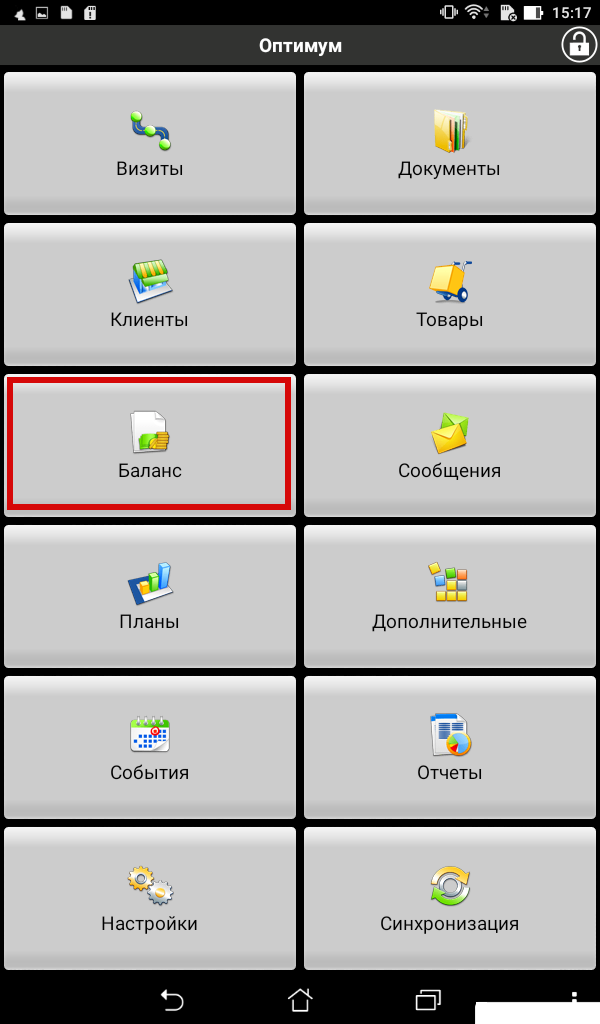
\includegraphics[width=0.8\linewidth]{scr5_1.png}}
	 		\ffigbox{\caption{Баланс}\label{pic:pic5_2}}%
	 		{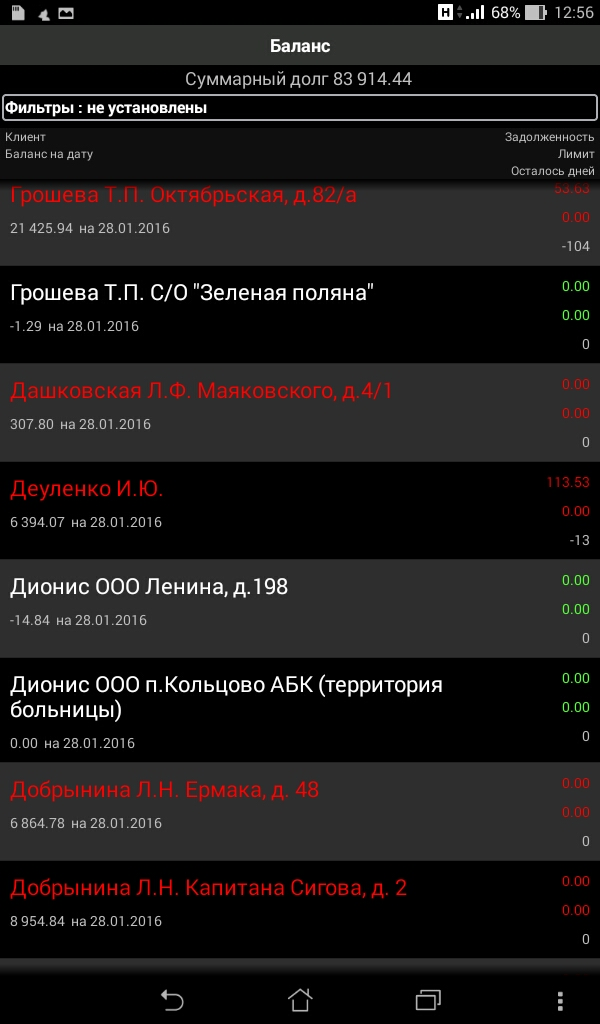
\includegraphics[width=0.8\linewidth]{scr5_2.jpg}}         
	 		\ffigbox{\caption{Подробный баланс}\label{pic:pic5_3}}%
	 		{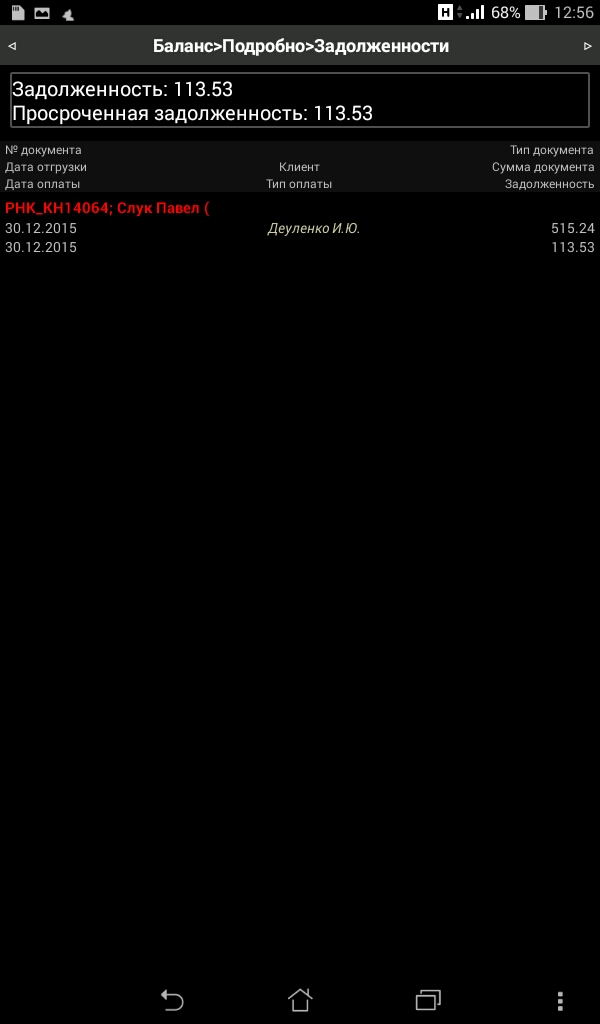
\includegraphics[width=0.8\linewidth]{scr5_3.jpg}}    
	 	\end{floatrow}
	 \end{figure}
	 
		
		
		

\end{enumerate}